\documentclass[10pt, a4paper, twocolumn]{jarticle}
%\documentclass[10pt, a4paper, twocolumn, uplatex]{jsarticle}
\usepackage{proceeding_bachelor}
\usepackage{tabularx}
\usepackage{booktabs}
\usepackage{multirow}
\usepackage{cite}
\usepackage{amsmath, amssymb}

% Title info. ======================================
\title{不確実性適応型損失関数による \\
頑健な医用画像セグメンテーション}

%%%%% 著者 %%%%%
\author{廣池 友哉}

%%%% 学籍番号 %%%%
\studentid{M243422}

%%%% 所属 %%%%
\affiliation{広島大学 大学院先進理工系科学研究科 情報科学プログラム}

%%%% 年度を書き換える %%%%
\proceedingname{2025年度修士論文中間発表予稿}

%%%% 卒論発表の日付を書く %%%%
\date{2025/9/19}


\begin{document}
%%%%%%%%%%%%% Header and Title %%%%%%%%%%%%%
\maketitle


%%% Please write your body text from here %%
\section{はじめに}
セマンティックセグメンテーションは,画像中の全てのピクセルに対し
物体のクラスのラベルを推定するタスクである.
特に医用画像の分野においては心臓MRIなどに用いられており,

しかし,医用画像セグメンテーションでは,画像全体に対する関心領域が
極小であるクラス不均衡という課題がある.

この課題に対処するため,少数クラスを考慮した学習を行うことができる損失関数が考案されてきた.
しかし,これらのアプローチでは検出難易度に関わらず誤差関数の形状が固定されており,
画像によって最適な重みづけがされていないことが課題だった.

そこで本研究では,検出難易度を画像毎に算出したものを学習に取り入れ,
誤差関数の形状を動的に変化させる手法を提案する.

本研究の最終的な目的は,画像毎のセグメンテーションの難易度指標を算出したものを学習に取り入れ,
誤差関数の形状を動的に変化させることである.その実現に向けた最初のステップとして,
本稿では難易度指標が学習が進むにつれてどのように推移するかを検証する.

\section{提案法}
図に提案法の概略図を示す.
提案法は,まず学習中に一定epoch毎に推論フェーズを挿入し,MC Dropoutにより複数枚の予測画像を得た後,
ピクセル単位で不確実性を計算し,画像全体の不確実性を難易度指標として算出する.

\subsection{PolyDice-1 Lossの説明}

\subsubsection{Polynomial Dice Lossの導出}
Dice Lossを拡張し多項式展開することを考える.
$W \times H$(pixel)の画像に対し,
予測画像を$\hat{\mathbf{y}} \in \mathbb R ^ {W \times H}$,
その画像に対する正解画像を$\mathbf{y} \in \mathbb R ^ {W \times H}$とし,
位置$i, j$における画素値をそれぞれ添字$i, j$を用いて$\hat{y}_{ij}, {y}_{ij}$と表現すると,Dice Lossは下記の式で示される.

\begin{equation}
  \mathcal{L}_{\text{Dice}}(\hat{\mathbf{y}}, \mathbf{y}) = 1 - \frac{2 \sum_{i=1}^{W} \sum_{j=1}^{H} \hat{y}_{ij} y_{ij}}{\sum_{i=1}^{W} \sum_{j=1}^{H}(\hat{y_{ij}} ^ 2 + y_{ij} ^ 2)}
\end{equation}

ここで予測画像$\hat{\mathbf{y}}$と正解画像$\mathbf{y}$をそれぞれ一次元のベクトル$\hat{\mathbf{y}} ^ {\prime}, {\mathbf{y}} ^ {\prime}$
に平坦化し,L2ノルム$\Vert \cdot \Vert$と内積$\langle \cdot, \cdot \rangle $を用いて
Dice Lossは次式のように表現することができる.
\begin{equation}
  \begin{aligned}
    \mathcal{L}_{\text{Dice}} &= 1 - \frac{2 \langle \hat{\mathbf{y}} ^ {\prime}, {\mathbf{y}} ^ {\prime} \rangle}{\Vert \hat{\mathbf{y}} ^ {\prime} \Vert ^ 2 + \Vert {\mathbf{y}} ^ {\prime} \Vert ^ 2} \\
    &= 1 - \frac{2 \Vert \hat{\mathbf{y}} ^ {\prime} \Vert \Vert {\mathbf{y}} ^ {\prime} \Vert}{\Vert \hat{\mathbf{y}} ^ {\prime} \Vert ^ 2 + \Vert {\mathbf{y}} ^ {\prime} \Vert ^ 2}
    \times \frac{\langle \hat{\mathbf{y}} ^ {\prime}, {\mathbf{y}} ^ {\prime} \rangle}{\Vert \hat{\mathbf{y}} ^ {\prime} \Vert \Vert {\mathbf{y}} ^ {\prime} \Vert}
  \end{aligned}
\end{equation}

この式において,$s = \frac{2 \langle \hat{\mathbf{y}} ^ {\prime}, {\mathbf{y}} ^ {\prime} \rangle}{\Vert \hat{\mathbf{y}} ^ {\prime} \Vert ^ 2 + \Vert {\mathbf{y}} ^ {\prime} \Vert ^ 2}$,
$\theta = \frac{\langle \hat{\mathbf{y}} ^ {\prime}, {\mathbf{y}} ^ {\prime} \rangle}{\Vert \hat{\mathbf{y}} ^ {\prime} \Vert \Vert {\mathbf{y}} ^ {\prime} \Vert}$とおくと,
Dice Lossは2つの成分,すなわちベクトル間の角度$\theta$に基づく方向成分(コサイン類似度)と,
ベクトルの大きさに基づくスケール成分$s$から構成されていることがわかる.
両方のベクトルが単位ノルムである場合、スケール成分$s=1$となり,Dice Lossはコサイン類似度そのものと一致する.
$\mathcal{L}_{\text{Dice}} = 1 - s \cos{\theta}$となる.
ここで,$\theta$は予測ベクトルと正解ベクトルのなす角であり,予測と正解が大きく変わらない,
つまり$\theta \approx 0$と仮定し,$\cos{\theta}$を$\theta = 0$まわりでテイラー展開すると以下のように近似できる.
\begin{equation}
  \cos{\theta} = 1 - \frac{\theta ^ 2}{2!} + \frac{\theta ^ 4}{4!} - \cdots
\end{equation}

スケール成分$s$を一定と仮定し,この近似式をDice Lossに代入して整理すると,以下のようになる.

\begin{equation}
  \begin{aligned}
  \mathcal{L}_{\text{Dice}} &= 1 - s \left(1 + \frac{1}{2!} \theta ^ 2 - \frac{1}{4!} \theta ^ 4 + \cdots\right) \\
  &= (1 - s) + s \left[\sum_{k = 1}^{\infty} \frac{(-1) ^ {k - 1}}{(2k)!} \theta ^ {2k}\right]
\end{aligned}
\end{equation}

ここで,各テイラー項の係数$\alpha_k$を$\alpha_k = \frac{(-1)^{k-1}}{(2k)!}$とすると,
Dice Lossを多項式展開したPolynomial Dice Lossは以下のように表現できる.

\begin{equation}
  \mathcal{L}_{\text{PolyDice}} = (1 - s) + s \sum_{k = 1}^{\infty} \alpha_k \theta ^ {2k}
\end{equation}

この損失関数を計算するために、角度$\theta$は以下のようにコサインの逆関数を用いて算出される.
\begin{equation}
  \theta = \arccos{\left(\frac{\langle \hat{\mathbf{y}} ^ {\prime}, {\mathbf{y}} ^ {\prime} \rangle}{\Vert \hat{\mathbf{y}} ^ {\prime} \Vert \Vert {\mathbf{y}} ^ {\prime} \Vert}\right)}
\end{equation}

このようにして,Dice Lossを幾何学的に解釈したうえでテイラー展開を用いることでPolynomial Dice Lossが導かれる.


\subsubsection{PolyDice-1 Lossの導出}
PolyLossのアプローチに倣い,多項式の次数に基づいてPolynomial Dice Lossのバリエーションを検討する.
まず,テイラー展開で得られた無限級数を第$K$項までで打ち切ることで,以下のような損失関数を定義する:

\begin{equation}
  \mathcal{L}_{\text{PolyDice-K}} = \mathcal{L}_{\text{PolyDice}} + s \sum_{k=1}^{K} \varepsilon_k \theta^{2k}
\end{equation}
%
%
しかし,これらのハイパーパラメータ$\varepsilon$を調整するのは難しく,
特に医用画像セグメンテーションでは交差検証による検証が用いられるため,このような複雑なチューニングは実用的ではない.
Leng らは,第$1$項($\theta ^ 2$)のみを調整するだけで十分な性能向上が得られることを示し,よりチューニングが容易なケース$K=1$の損失関数を提案している.
これに従い,以下のようにPolyDice-1 Lossを定義する.

\begin{equation}
  \mathcal{L}_{\text{PolyDice-1}} = (1 - s) + s(\alpha_1 + \epsilon_1) \theta^2
\end{equation}

\newpage

\section{図表について}
\subsection{図の挿入}
図の使用例を次に示します.
\newline

Dice Lossは予測画像と正解画像との類似度を測るDice Indexに基づいて定義される.
$W \times H$(pixel)のモデルの予測画像を$\hat{\mathbf{y}} \in \mathbb R ^ {W \times H}$,
その画像に対する正解画像を$\mathbf{y} \in \mathbb R ^ {W \times H}$とすると,
Dice Lossは下記の式で示される.

\begin{equation}
  \mathcal{L}_{\text{Dice}}(\hat{\mathbf{y}}, \mathbf{y}) = 1 - \frac{2 \sum_{i=1}^{W} \sum_{j=1}^{H} \hat{y}_{ij} y_{ij}}{\sum_{i=1}^{W} \sum_{j=1}^{H} (aa \hat{y_{ij}} ^ 2 + y_{ij} ^ 2)}
\end{equation}


東広島キャンパスでは,図\ref{fig:campus}に示すように,
初夏にはアメリカ楓の美しい並木が緑に輝く.
%
\begin{figure}[t]
	\begin{center}
		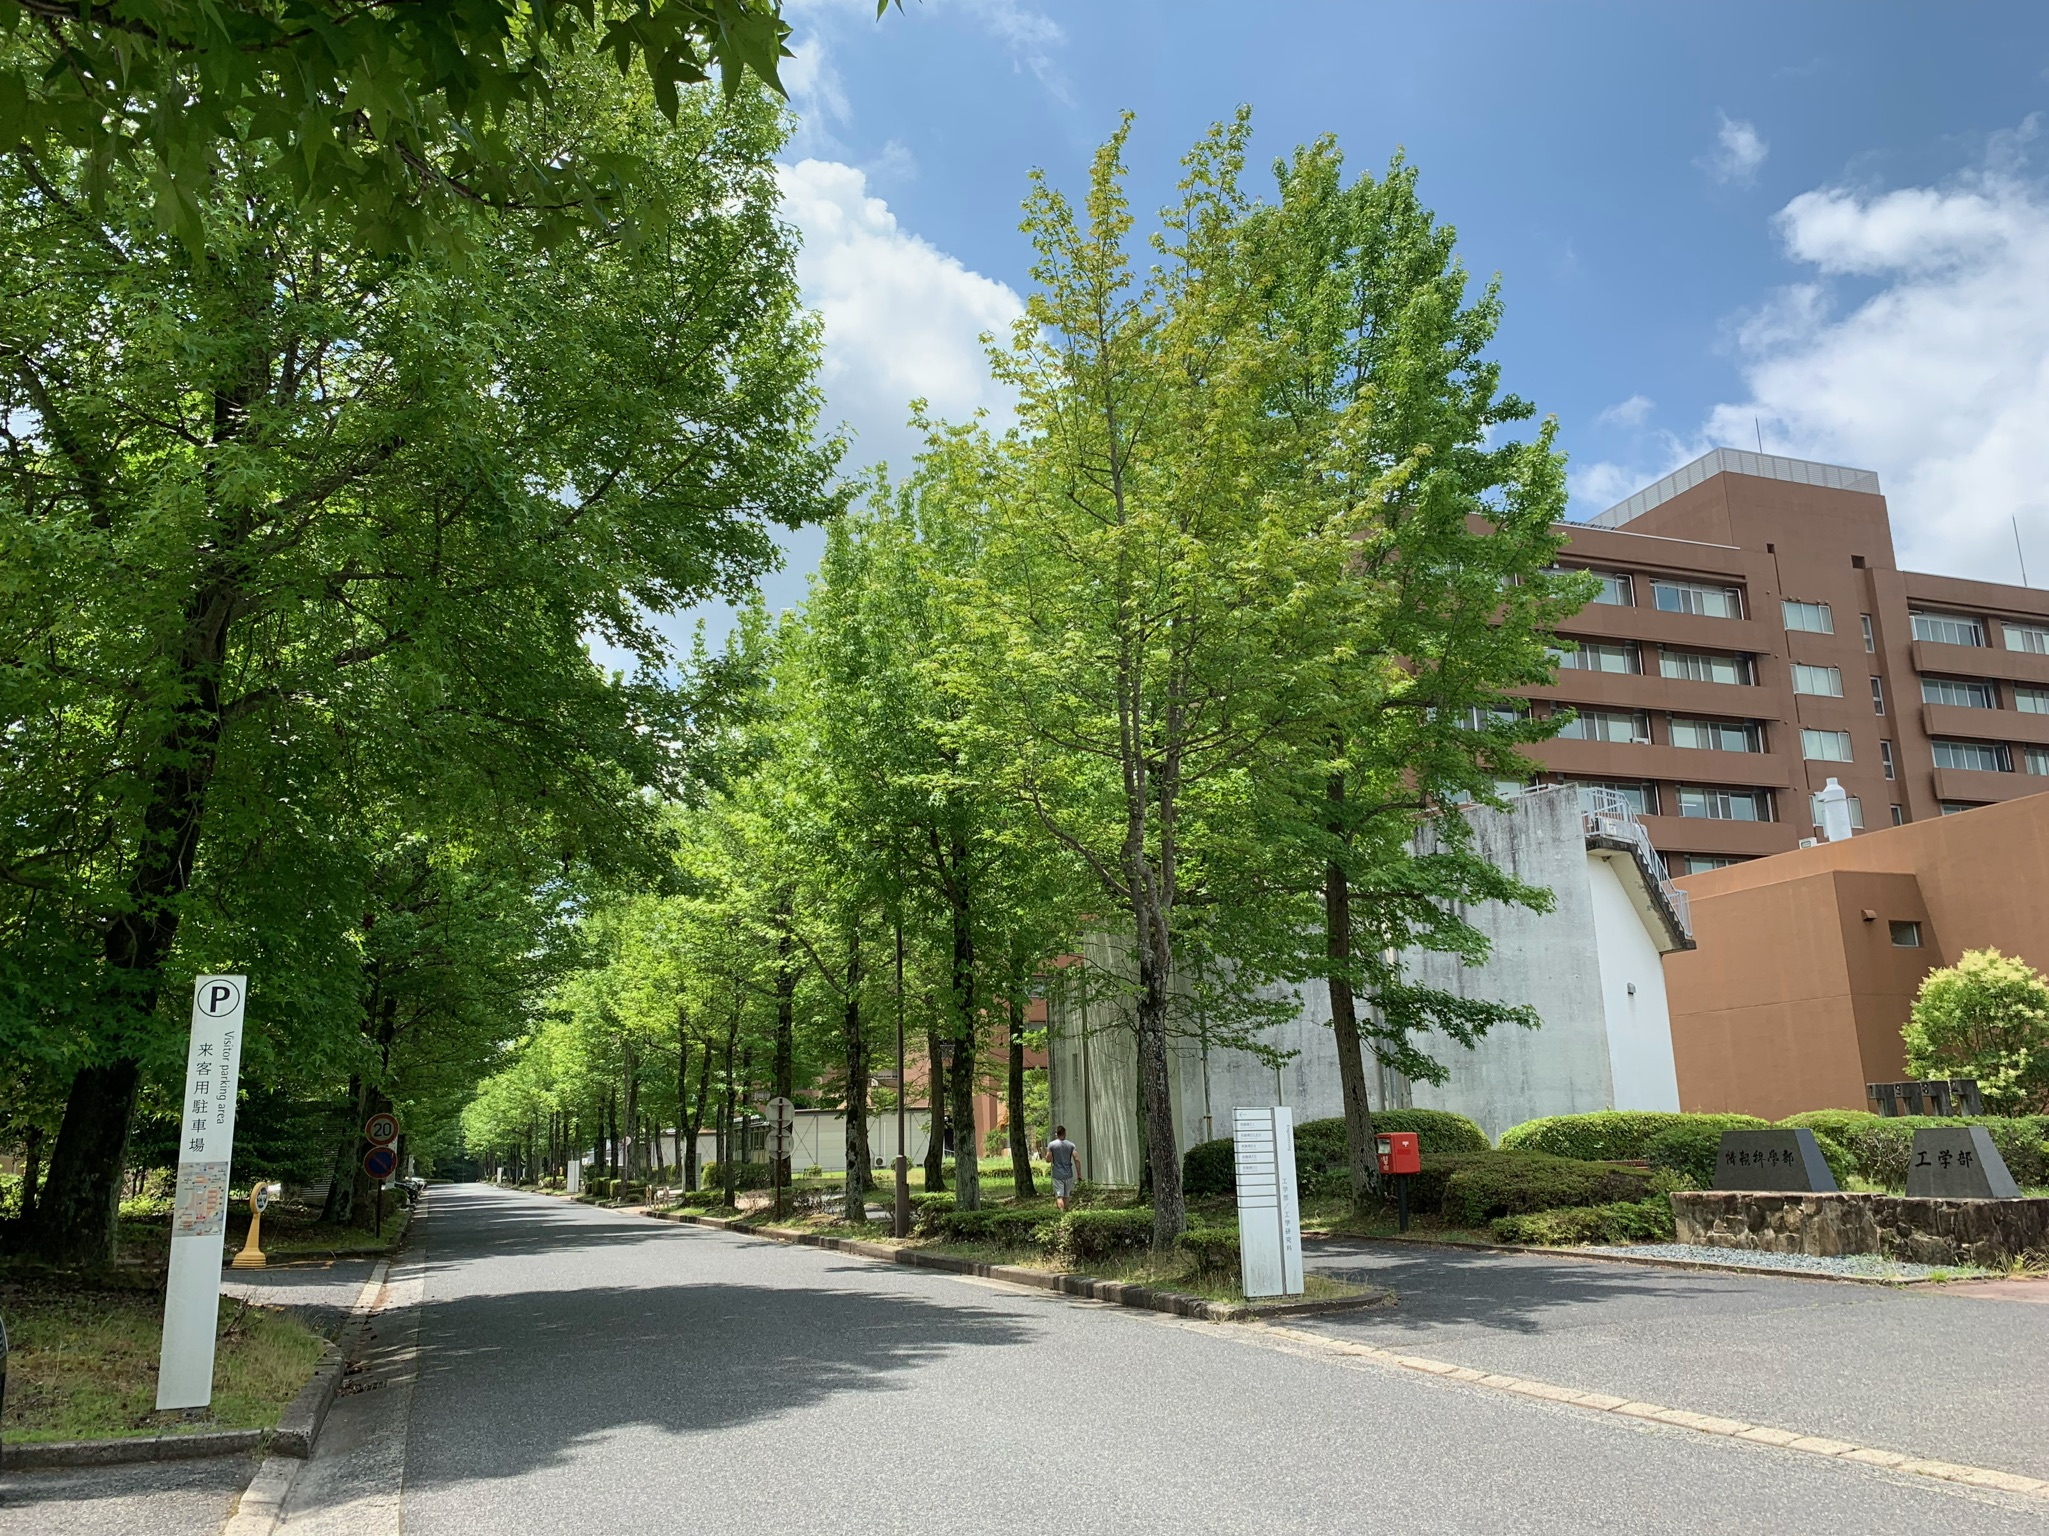
\includegraphics[width=0.95\hsize]{figure/campus.jpg}
	\end{center}
	\vspace{-12pt} %図とキャプションとの間隔調整
	\caption{東広島キャンパスのアメリカ楓並木}
	\label{fig:campus}
\end{figure}
%
\newline

Minkowski Islandは4つのMinkowski Sausage (Quadratic type 2 curve) を
正方形状に配置したフラクタル図形である(図\ref{fig:fractal}参照).
%
\begin{figure}[b]
	\begin{center}
		
\includegraphics[scale=1]{figure/fractal.pdf}
	\end{center}
	\vspace{-12pt} %図とキャプションとの間隔調整
	\caption{Minkowski Island}
	\label{fig:fractal}
\end{figure}
%
\newpage

\subsection{表の作成}
表の記入例を次に示します.

コースティックフォトンマップには,光源から放出されたフォトンが拡散反射面に到達する前に,
1回以上鏡面反射あるいは透過したフォトンの情報が格納される.
すなわち,表\ref{tab:path_notation}に示す表記法を用いれば,
{\tt LS+D}の経路をたどったフォトンの位置,放射束,入射方向が記録される.
%
\begin{table}[t]
  \begin{center}
  \caption{光の経路の表記法}
  \label{tab:path_notation}
  \begin{tabular}{l l | l l} \toprule
    {\tt L} & 光源 & {\tt (k)+} & {\tt k}が1回かそれ以上起きる \\ 
    {\tt E} & 視点 & {\tt (k)*} & {\tt k}が0回かそれ以上起きる \\
    {\tt S} & 鏡面反射 & {\tt (k)?} & {\tt k}が0回か1回起きる \\ 
    {\tt D} & 拡散反射 & {\tt (k|k')} & {\tt k}あるいは{\tt k'}が起きる \\ \bottomrule
  \end{tabular}
  \end{center}
\end{table}
%
\newline

\section{文献引用}
文献引用の例を次に示します.
\newline

レンダリング方程式(rendering equation)~\cite{kajiya1986rendering}は,算出すべき放射輝度$L$が式の両辺に表れた積分方程式となっている.

フォトンマッピング法~\cite{jensen2001realistic}では2段階のレイトレーシングを行うことによりレンダリング方程式を解く.


\section{まとめ}
修士論文中間発表予稿の様式を示しました.

%%%%% 参考文献(BibTeXを使う場合) %%%%%
\bibliographystyle{bibstyle} % bstファイルを設定
\bibliography{references} % bibファイルを読み込み

%%%%% 参考文献(直接書く場合) %%%%%
% \begin{thebibliography}{9} %\footnotesize
    % \bibitem{kajiya1986rendering}
    % J.~T. Kajiya,
    % \newblock ``The rendering equation,''
    % \newblock in {\em Proceedings of the 13th Annual Conference on Computer
    %   Graphics and Interactive Techniques}, pp. 143--150, 1986.
    
    % \bibitem{jensen2001realistic}
    % H.~W. Jensen,
    % \newblock {\em Realistic image synthesis using photon mapping}, vol. 364,
    % \newblock Ak Peters Natick, 2001.
% \end{thebibliography}

\end{document}